\chapter{Predictieve modellen}
\label{cha:D:predictieve-modellen}

\section{Introductie}
\label{sec:D:pm-introductie}
In dit hoofdstuk leggen we uit wat een predictief model inhoudt en hoe deze worden opgebouwd. We zullen hiervoor twee concrete voorbeelden gebruiken: logistieke regressie en cox survival modellen. Verder leggen we ook het concept van regularisatie uit, dit zal belangrijk blijken in het volgende hoofdstuk over integratie strategie\"en. Tenslotte zullen we ook kort uitleggen wat validatie inhoudt.

\section{Wat is een predictief model?}
\label{sec:D:pm}
Een predictief model is een relatie tussen input variabelen en een doelfunctie (doel variabele). De taak van een predictief model is om een waarde te voorspellen voor de doelfunctie, gegeven een set van waarden voor de input variabelen. Bijvoorbeeld: we kunnen een predictief model bouwen dat de relatie probeert voor te stellen tussen een datum en de gemiddelde temperatuur op die dag. De input is hier de datum, de doelfunctie (of output) is de gemiddelde temperatuur voor die dag. We kunnen ons inbeelden dat er tussen deze twee variabelen een verband bestaat. Een datum ergens in de zomer zal namelijk een relatief hoge gemiddelde temperatuur opleveren, en een dag in de winter een relatief lage temperatuur. We weten dit omdat we jarenlang ervaring hebben opgebouwd en ons hebben gerealizeerd dat het in de zomer normaal warm is en in de winter koud. Dit is precies wat we proberen te vatten met een predictief model, het onderliggende patroon. En de manier om daartoe te komen is door ervaring op te bouwen. Op eenzelfde manier gaan we proberen het model ervaring te laten opbouwen, we noemen dit dan 'het model trainen'. We gaan het model voorbeelden tonen van wat we willen dat het model leert, en het model zal hieruit leren en intern een representatie opbouwen om zijn kennis voor te stellen. In het eerder gegeven voorbeeld zouden we, om het model te trainen, een hele lijst met data en de corresponderende gemiddelde temperatuur voor die dag tonen aan het model, dit noemen we de training set. Het model zal dan intern een representatie opbouwen van zijn kennis en als alles goed verloopt zal deze representatie inderdaad weergeven dat het in de zomer normaal warmer is en in de winter normaal kouder. Welke representatie het model intern gebruikt is een keuze die we zelf maken, en hangt af van het type van patronen dat we willen representeren en dus van de relatie die we denken dat er bestaat tussen de input en de doelfunctie. Er zijn talloze representaties mogelijk, in dit thesis focussen we ons op lineaire representaties. Dit wil zeggen dat we veronderstellen dat we een lineaire combinatie kunnen maken van de input variabelen, en daarmee accuraat de doelfunctie kunnen benaderen. Afhankelijk van het type van de doelfunctie die we willen benaderen zijn hier echter nog verschillende methoden voor, in de volgende secties bekijken we twee concrete voorbeelden: logistieke regressie en cox modellen.

\section{Logistieke regressie}
\label{subsec:D:pm-logistieke-regressie}
In logistieke regressie maken we twee veronderstellingen. De eerste is dat er een lineair verband bestaat tussen de input variabelen en de doelfunctie. De tweede is dat, in de training set, de waarden van de doelfunctie het resultaat zijn van een binomiaalverdeling. Denk hierbij bijvoorbeeld aan het genezen of niet-genezen van een kankerpati\"ent, in onze training set zullen we enkel de waarden 'genezen' en 'niet-genezen' aantreffen, maar we weten dat onderliggend deze waarden gegenereerd zijn met een bepaalde probabiliteit van overleving. De taak in logistieke regressie (en dus van ons predictief model) is om deze onderliggende probabiliteit te schatten. Stel dat we N voorbeeld datapunten hebben waarbij elk datapunt M input variabelen bevat, dan kunnen we logistieke regressie als volgt neerschrijven:
\begin{equation}
\begin{split}
\hat{y}_{n} = \theta(\sum_{i=1}^{M}w_{i}x_{in})= \theta(\bm{w^{T}x_{n}}) \qquad for\ n=1..N
\end{split}
\end{equation}
hierin is
\begin{itemize}
	\item $\hat{y}_{n}$ is de geschatte waarde voor de probabiliteit voor datapunt $n$
	\item $w_{i}$ is de model parameter (co\"effici\"ent) voor input variabele $i$
	\item $x_{in}$ is de waarde voor input variabele $i$ voor datapunt $n$
	\item $\bm{w^{T}x}$ is de vector notatie voor het inwendig product van $\bm{w}$ en $\bm{x}$
	\item $\theta(x)$ is de logistieke functie. Een voorbeeld voor deze function is $\frac{e^{x}}{1+e^{x}}$
\end{itemize}
Deze formule geeft weer dat, gegeven een input vector $\bm{x_{n}}$, ons model in staat is om zijn interne kennis (met representatie $\bm{w}$) te gebruiken om een waarde te voorspellen ($\hat{y}_{n}$) voor de probabiliteit. De functie $\theta$ is de logistieke functie, deze functie is een mapping van de re\"ele getallen naar het bereik $[0..1]$ en zorgt ervoor dat we het resultaat kunnen interpreteren als een probabiliteit.

\section{Cox proportionele risico modellen}
Het volgende type modellen dat we bespreken valt onder de noemer van survival (overlevings-) modellen. Bij deze modellen proberen we de de tijd te schatten tot het voorkomen van een bepaald event op basis van de input variabelen. In ons geval is het event dat we bestuderen het overlijden van patienten aan kanker, vanaf nu zullen we dit ook zo behandelen. De doelfunctie wordt daarom ook wel de overlevingsfunctie genoemd. Om overlevingsfuncties te plotten worden vaak kaplan-meier curves gebruikt, op figuur \ref{fig:D:cox-example-kaplan-meier} worden twee voorbeeld overlevingsfuncties getoond.	
\begin{figure}
	\centering
	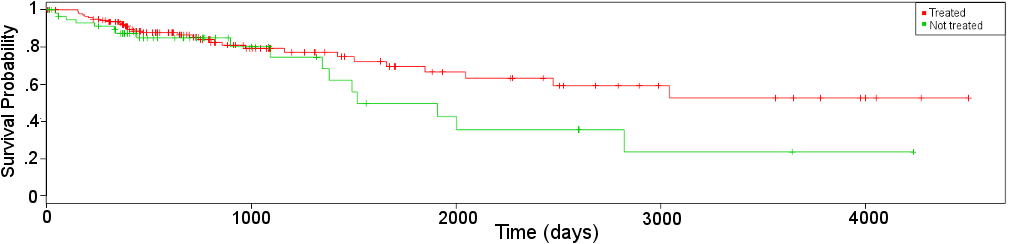
\includegraphics[scale=0.4]{images/example_kaplan_meier_curve}
	\caption{Voorbeeld kaplan-meier survival curves. De X-as geeft de tijd weer, de Y-as geeft de kans weer op overleving.}
	\label{fig:D:cox-example-kaplan-meier}
\end{figure}
Bij overlevingsanalyze wordt echter ook vaak gebruik gemaakt van de zogenaamde hazard (of risico) functie. Deze functie geeft weer wat het risico is dat op een gegeven tijdstip het event zich voordoet. In het cox proportionele risico model dat we zullen gebruiken wordt deze risico functie als volgt genoteerd:
\begin{equation}
\begin{split}
\lambda_{i}(t) = \lambda_{0}(t)e^{X_{i1}\beta_{1} + ... + X_{iN}\beta_{N}}
\end{split}
\end{equation}
where
\begin{itemize}
	\item $\lambda_{i}(t)$ is het risico op overlijden voor pati\"ent i op tijdstip t.
	\item $\lambda_{0}(t)$ is de baseline risico op tijdstip t, dit is het risico op overlijden zonder enige invloed van de input variabelen.
	\item $X_{i1} ... X_{iN}$ zijn de waarden voor de input variabelen voor pati\"ent i.
	\item $\beta_{1} ... \beta_{N}$ zijn de waarden voor de parameters van het model (de kennis representatie).
\end{itemize}
Een tweede interessant concept is wat met noemt de risico-verhouding (hazard ratio). Dit is de verhouding van twee risico functies:
\begin{equation}
\label{eq:D:cox-hazard-ratio}
\begin{split}
\frac{\lambda_{i}(t)}{\lambda_{j}(t)} 
= \frac{\lambda_{0}(t)e^{X_{i1}\beta_{1} + ... + X_{iN}\beta_{N}}}{\lambda_{0}(t)e^{X_{j1}\beta_{1} + ... + X_{jN}\beta_{N}}}
= e^{(X_{i1}-X_{j1})\beta_{1} + ... + (X_{iN}-X_{jN})\beta_{N}}
\end{split}
\end{equation}
Merk op dat de vorm van de risico functie een keuze is die we zelf hebben gemaakt, door te kiezen voor cox proportionele risico modellen. Deze keuze heeft twee heel belangrijke gevolgen die duidelijk worden in de formule van de risico-verhouding (\ref{eq:D:cox-hazard-ratio}). Het eerste gevolg is dat risico-verhoudingen onafhankelijk zijn van de tijd. Dit wil zeggen dat de risico-verhouding tussen twee pati\"nten dus niet verandert doorheen de tijd. Vandaar ook de naam 'proportionele risico modellen'. Het tweede gevolg is dat veranderingen in de input variabelen een multiplicatief effect hebben op het risico. Dit kunnen we ook zien in formule \ref{eq:D:cox-hazard-ratio}, maar is nog duidelijker als we de risico-verhouding neerschrijven met in de noemer het risico voor een pati\"ent met bepaalde waarden voor de input variabelen, en in de teller het risico voor een pati\"ent met exact dezelfde input waarden, behalve voor 1 variabele $X_{j}$ een verhoging met 1:
\begin{equation}
\begin{split}
\frac{\lambda(t|X_{j}+1)}{\lambda(t|X_{j})} = e^{(X_{j}+1-X_{j})\beta_{j}} = e^{\beta_{j}}
\end{split}
\end{equation}
We zien dus dat een verhoging met 1 voor een input variabele, het risico doet veranderen met $e^{\beta_{j}}$, de exponenti\"ele van de bijhorende co\"effici\"ent.

\subsection{Het predictief overlevingsmodel}
Net zoals bij logistieke regressie hebben we hier dus te maken met een set gewichten die onze kennis representatie voorstellen. We zullen ook heel analoog een iteratief algoritme gebruiken om deze gewichten te bepalen. We zullen het model een hele reeks voorbeeld datapunten tonen (input variabelen met bijhorende overlevingskans) om zo het model ervaring te laten opbouwen en op die manier zo goed mogelijk de overlevingskansen van pati\"enten te laten schatten.

\section{Regularizatie}
Een belangrijk concept dat we moeten toevoegen aan onze modellen is regularizatie. Herinner je uit sectie \ref{sec:D:pm} dat we een predictief model opbouwen door het een reeks voorbeeld datapunten te geven om het op die manier zijn interne representatie van de kennis te laten opbouwen. In beide voorbeeld modellen die we hebben gezien is deze representatie en set van gewichten. Het concept van regularizatie houdt in dat we een of meerdere beperkingen gaan opleggen aan deze gewichten. Het doel hiervan is om bepaalde modellen (bepaalde combinaties van gewichten) te prefereren boven anderen. De onderliggende gedachte is dat we gaan trachten van simpele modellen te bekomen, die een vloeiende functie voorstellen. We doen dit om te voorkomen dat het model patronen gaat vinden die er eigenlijk niet zijn of die enkel het resultaat zijn van ruis is de gegevens. Er zijn verschillende beperkingen mogelijk die we kunnen opleggen, en elk krijgen ze hun eigen naam: de ridge penalty, de lasso penalty en het elastisch-net pentalty.
\subsection{Ridge penalty}
Bij de ridge penalty (ook wel $L_{2}$ panalty genoemd) is de beperking die we opleggen de volgende:
$$
\sum_{i=1}^{N}w_{i}^{2} \leq C
$$
Deze beperking zal ervoor zorgen dat gewichten klein worden gehouden, en het dus onmogelijk wordt dat een gewicht extreem groot wordt relatief ten opzichte van de andere gewichten.
\subsection{Lasso penalty}
Bij de lasso penalty (ook wel $L_{1}$ penalty genoemd) is de beperking:
$$
\sum_{i=1}^{N}\lvert w_{i}\rvert \leq C
$$
Deze beperking heeft ook als gevolg dat de gewichten klein worden gehouden, maar heeft als extra dat gewichten ook effectief 0 worden indien ze niet belangrijk genoeg zijn in het model. We noemen dit daarom ook 'variabele selectie'. Gebruik van de lasso penalty heeft als gevolg dat het resulterende model vaak minder parameters gebruikt, omdat het enkel deze parameters gebruikt die echt belangrijk zijn. Deze techniek zal zeer belangrijk blijken bij een van de integratie technieken die later worden besproken.
\subsection{Elastisch-net penalty}
Bij het elastisch-net penalty is de beperking een combinatie van de ridge en lasso penalties:
$$
\alpha \sum_{i=1}^{N}w_{i}^{2} + (1-\alpha)\sum_{i=1}^{N}\lvert w_{i}\rvert \leq C
$$
Deze methode heeft daarom ook eigenschappen van zowel ridge als lasso, en met de parameter $\alpha$ kan men kiezen hoezeer men wil aanleunen bij een van de twee technieken. Dit vormt als het ware een gulden middenweg.
\subsection{De parameter $\lambda$}
Wanneer met regularizatie echter toepast op een concreet model, zal men altijd het optimalisatie probleem met beperking proberen omvormen naar een equivalent optimalisatie probleem zonder beperking. Bij deze omvorming introduceert men dan meestal een parameter $\lambda$ die als vervanging dient voor de parameter $C$ in bovenstaande beperkingen. $\lambda$ kan men zien als de hoeveelheid regularizatie die men wil gebruiken. Hoe groter $\lambda$ hoe sterker de beperking en dus hoe kleiner $C$. Hoe kleiner $\lambda$, hoe minder regularizatie, hoe groter $C$.

\section{Validatie}
Het laatste concept dat we moeten behandelen is validatie. Dit zal ons toelaten om een getraind model te evalueren. Bij validatie delen we onze dataset op in twee delen: een training set en een validatie set. De training set kennen we reeds, deze datapunten zullen we gebruiken om een model te trainen. Merk op dat we nu echter nog datapunten over hebben die niet gebruikt werden voor de training, dit is de validatie set. We zullen het getrainde model vragen om voor deze datapunten een predictie te berekenen voor de output variabelen. We kennen van de datapunten in de validatie set echter de correcte output waarde. We kunnen vervolgens dus de output van ons predictief model vergelijken met de juiste waarde, en op die manier een idee krijgen hoe goed ons predictief model presteert. \\ \\
Merk echter op dat de training set die we gebruiken om het model te trainen kleiner is dan de volledige dataset waarover we beschikken. We houden inderdaad de datapunten in de validatie set opzij. We willen echter zoveel mogelijk datapunten gebruiken om te trainen, want dan bekomen we een beter model. Langs de andere kant willen we ook genoeg datapunten in de validatie set om een goed beeld te krijgen van de performantie van het bekomen model. Een oplossing voor deze contradictie is cross-validatie. Bij cross-validatie delen we onze dataset op in K (vaak 10) gelijke stukken. We gebruiken 1 van de K stukken als validatie set, en de andere K-1 stukken als training set. We herhalen dit proces K keren, waarbij we iedere keer een ander stuk nemen als validatie set. Op die manier hebben we op het einde voor elk datapunt in onze dataset een predictie. Deze predicties kunnen we dan vergelijken met de echte waarden en dit zal ons een redelijk goed beeld geven van de performantie van het model dat we zouden bekomen indien we op de volledige dataset zouden trainen.
%%% Local Variables: 
%%% mode: latex
%%% TeX-master: "thesis"
%%% End: 
